\documentclass[tikz,border=8pt]{standalone}
\usepackage[T1]{fontenc}
\IfFileExists{libertine.sty}{\usepackage{libertine}}{}
\IfFileExists{inconsolata.sty}{\usepackage[scaled=0.94]{inconsolata}}{}
\usetikzlibrary{arrows.meta,calc,positioning}

\definecolor{ink}{RGB}{31,40,50}
\definecolor{muted}{RGB}{101,112,124}
\definecolor{hairline}{RGB}{216,222,228}
\definecolor{panel}{RGB}{248,250,252}
\definecolor{navy}{RGB}{38,91,145}
\definecolor{navyfill}{RGB}{235,243,250}
\definecolor{amber}{RGB}{184,112,29}
\definecolor{amberfill}{RGB}{252,244,231}
\definecolor{textgreen}{RGB}{80,120,99}

\begin{document}
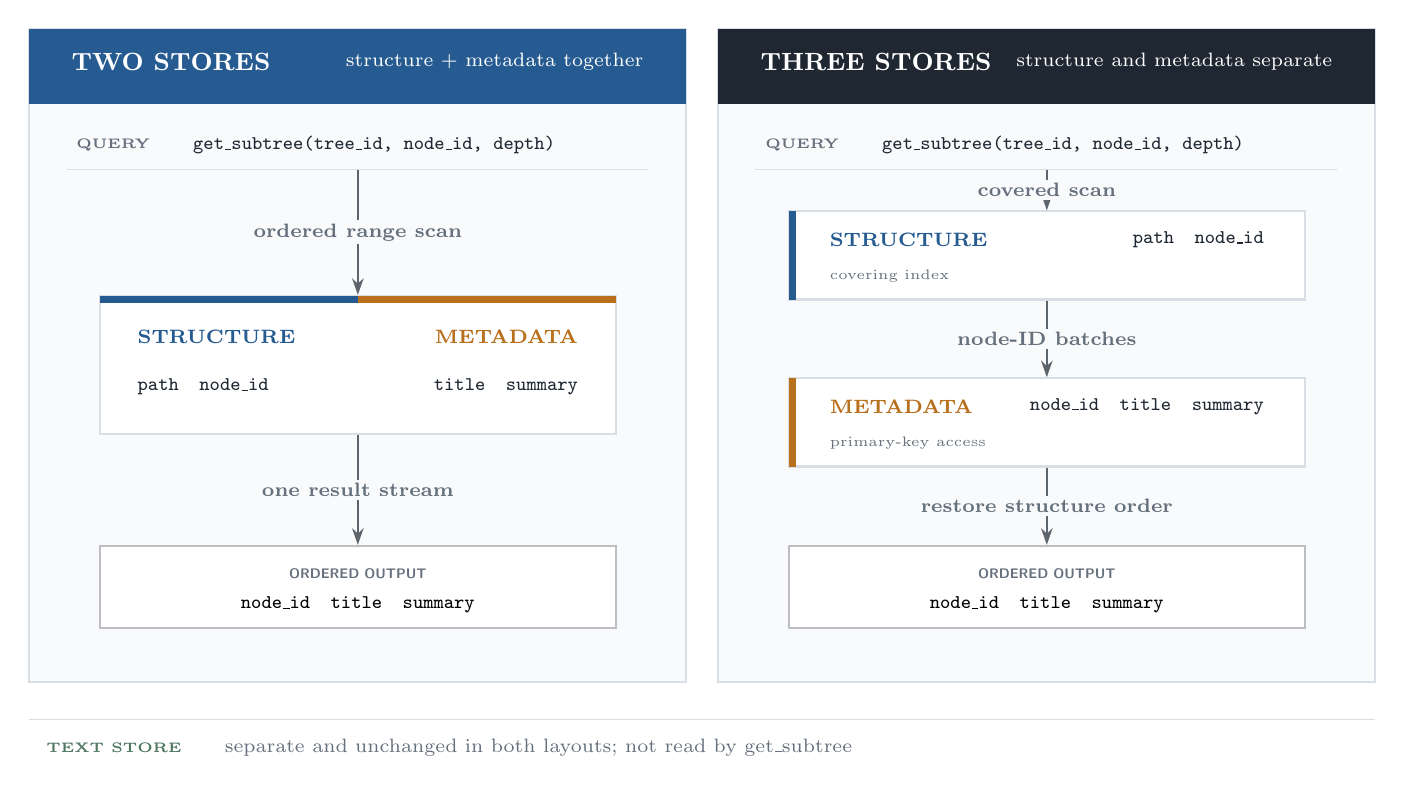
\begin{tikzpicture}[
  x=1cm,y=1cm,
  font=\sffamily,
  flow/.style={-{Stealth[length=2.1mm,width=1.45mm]}, draw=ink!72,
               line width=0.82pt},
  store/.style={draw=hairline, fill=white, line width=0.8pt},
  code/.style={font=\scriptsize\ttfamily, text=ink},
  stage/.style={font=\scriptsize\bfseries, text=muted, fill=panel,
                inner xsep=2.2pt, inner ysep=1.2pt},
  output/.style={draw=ink!30, fill=white, line width=0.8pt,
                 minimum width=6.55cm, minimum height=0.82cm,
                 align=center}
]

% Flat comparison panels.
\fill[panel] (0,0.85) rectangle (8.35,9.15);
\draw[hairline, line width=0.75pt] (0,0.85) rectangle (8.35,9.15);
\fill[panel] (8.75,0.85) rectangle (17.10,9.15);
\draw[hairline, line width=0.75pt] (8.75,0.85) rectangle (17.10,9.15);

% Panel headings use a compact editorial treatment instead of diagram cards.
\fill[navy] (0,8.20) rectangle (8.35,9.15);
\node[anchor=west, font=\small\bfseries, text=white]
  at (0.42,8.73) {TWO STORES};
\node[anchor=east, font=\scriptsize, text=white!80]
  at (7.93,8.73) {structure + metadata together};

\fill[ink] (8.75,8.20) rectangle (17.10,9.15);
\node[anchor=west, font=\small\bfseries, text=white]
  at (9.17,8.73) {THREE STORES};
\node[anchor=east, font=\scriptsize, text=white!76]
  at (16.68,8.73) {structure and metadata separate};

% Identical query at the top of both lanes.
\node[anchor=west, font=\tiny\bfseries, text=muted] (ql2)
  at (0.48,7.67) {QUERY};
\node[code, anchor=west] (q2) at ([xshift=3mm]ql2.east)
  {get\_subtree(tree\_id, node\_id, depth)};
\draw[hairline] (0.48,7.36) -- (7.87,7.36);

\node[anchor=west, font=\tiny\bfseries, text=muted] (ql3)
  at (9.23,7.67) {QUERY};
\node[code, anchor=west] (q3) at ([xshift=3mm]ql3.east)
  {get\_subtree(tree\_id, node\_id, depth)};
\draw[hairline] (9.23,7.36) -- (16.62,7.36);

% Two-store lane: one combined record and one ordered range scan.
\node[store, minimum width=6.55cm, minimum height=1.75cm]
  (combined) at (4.18,4.88) {};
\fill[navy] ([xshift=-3.275cm,yshift=0.875cm]combined.center)
  rectangle ([xshift=0cm,yshift=0.79cm]combined.center);
\fill[amber] ([xshift=0cm,yshift=0.875cm]combined.center)
  rectangle ([xshift=3.275cm,yshift=0.79cm]combined.center);
\node[anchor=west, font=\scriptsize\bfseries, text=navy]
  at ([xshift=-2.92cm,yshift=0.36cm]combined.center) {STRUCTURE};
\node[anchor=east, font=\scriptsize\bfseries, text=amber]
  at ([xshift=2.92cm,yshift=0.36cm]combined.center) {METADATA};
\node[anchor=west, code]
  at ([xshift=-2.92cm,yshift=-0.28cm]combined.center)
  {path\quad node\_id};
\node[anchor=east, code]
  at ([xshift=2.92cm,yshift=-0.28cm]combined.center)
  {title\quad summary};

\draw[flow] (4.18,7.36) -- (combined.north)
  node[stage, midway] {ordered range scan};

\node[output] (out2) at (4.18,2.06) {
  \begin{tabular}{c}
    {\tiny\bfseries\color{muted} ORDERED OUTPUT}\\[-1pt]
    {\scriptsize\ttfamily node\_id\quad title\quad summary}
  \end{tabular}};
\draw[flow] (combined.south) -- (out2.north)
  node[stage, midway] {one result stream};

% Three-store lane: covered ID scan, batched key lookup, then ordered merge.
\node[store, minimum width=6.55cm, minimum height=1.12cm]
  (structure) at (12.93,6.27) {};
\fill[navy] ([xshift=-3.275cm,yshift=0.56cm]structure.center)
  rectangle ([xshift=-3.18cm,yshift=-0.56cm]structure.center);
\node[anchor=west, font=\scriptsize\bfseries, text=navy]
  at ([xshift=-2.88cm,yshift=0.20cm]structure.center) {STRUCTURE};
\node[anchor=east, code]
  at ([xshift=2.88cm,yshift=0.20cm]structure.center) {path\quad node\_id};
\node[anchor=west, font=\tiny, text=muted]
  at ([xshift=-2.88cm,yshift=-0.26cm]structure.center) {covering index};

\node[store, minimum width=6.55cm, minimum height=1.12cm]
  (metadata) at (12.93,4.15) {};
\fill[amber] ([xshift=-3.275cm,yshift=0.56cm]metadata.center)
  rectangle ([xshift=-3.18cm,yshift=-0.56cm]metadata.center);
\node[anchor=west, font=\scriptsize\bfseries, text=amber]
  at ([xshift=-2.88cm,yshift=0.20cm]metadata.center) {METADATA};
\node[anchor=east, code]
  at ([xshift=2.88cm,yshift=0.20cm]metadata.center)
  {node\_id\quad title\quad summary};
\node[anchor=west, font=\tiny, text=muted]
  at ([xshift=-2.88cm,yshift=-0.26cm]metadata.center) {primary-key access};

\draw[flow] (12.93,7.36) -- (structure.north)
  node[stage, midway] {covered scan};
\draw[flow] (structure.south) -- (metadata.north)
  node[stage, midway] {node-ID batches};

\node[output] (out3) at (12.93,2.06) {
  \begin{tabular}{c}
    {\tiny\bfseries\color{muted} ORDERED OUTPUT}\\[-1pt]
    {\scriptsize\ttfamily node\_id\quad title\quad summary}
  \end{tabular}};
\draw[flow] (metadata.south) -- (out3.north)
  node[stage, midway] {restore structure order};

% Text is deliberately outside both subtree paths.
\draw[hairline] (0,0.38) -- (17.10,0.38);
\node[anchor=west, font=\tiny\bfseries, text=textgreen] (textlabel)
  at (0.10,0.02)
  {TEXT STORE};
\node[anchor=west, font=\scriptsize, text=muted]
  at ([xshift=3mm]textlabel.east)
  {separate and unchanged in both layouts; not read by get\_subtree};

\end{tikzpicture}
\end{document}
